\section{Kinematic calculation}\label{Kinematic calculation}

We want to calculate the maximum possible momentum/energy of $\pi^+$, in the lab frame, for the reaction $p(\gamma,\pi^{+})\pi{^0}n$, for a given photon energy, which we will assume to be equal to the beam energy ($E_{beam}$). For the sake of simplicity, first this calculation can be done for the reaction $p(\gamma,\pi^{+})n$ (which is actually the reaction we are interested in using as a tagged neutron source to calibrate HCal neutron detection efficiency), and then extend it to the first reaction.

\subsection{Formalism}

\subsubsection{Consider reaction $p(\gamma,\pi^{+})n$}

Define the four-momenta of the particles involved in the reaction as $p_{\gamma}$, $p_{p}$, 
$p_{\pi^{+}}$, and $p_{n}$. Where we can write values before the reaction as,\\
$p_{\gamma} = (E_{\gamma}, 0, 0, E_{\gamma})$ and $p_{p} = (m_p, 0, 0, 0)$ \\ are the four momenta of the photon and the proton before the scattering reaction. In order for the momentum of resulting $\pi^+$ to be maximum, we can argue that the $\pi^+$ must be ejected in the +Z/beam direction and the neutron in the -Z/opposite to the beam direction. This situation is easier to evaluate in the CM frame and find the momentum of $\pi^+$ there and then Lorentz transform that momentum into the lab frame. In the CM frame, let's assume that the $\pi^+$'s 3-momentum is $\vec{P}'_{\pi^+}$ and neutron 3-momentum is $\vec{P}'_{n}$. But because we are at CM frame $\vec{P}'_{\pi^+}+\vec{P}'_{n}=0$. Here the direction of the $\vec{P}'_{\pi^+}$ vector should be in the +Z/+Z$'$. We will identify S as our lab frame and S$'$ as our CM frame. Therefore we can use prime notation for all the quantities measured in the CM frame.\\
Then we can use the Mandelstam `$s$' variable, which is a Lorentz invariant to simplify our calculation. 
For a two-body scattering reaction of the type A(B,C)D,\\

\vspace{0.1cm}
%\centering
\begin{equation}
   s = (p_A + p_B)^2
\end{equation}
%\vspace{0.2cm}
Therefore, from the lab frame, we can write $s$ as, 
\begin{equation}\label{equ: Mandelstam s in lab fram}
    s = (p_{\gamma} + p_{p})^2 = p_{\gamma}^2+p_{p}^2+2p_{\gamma}p_{p} = m_p^2 + 2E_{\gamma}m_p
\end{equation}
Then, in CM frame the total energy can be expressed as,
\begin{equation}\label{equ: Mandelstam s in CM frame}
 E'_{tot} = \sqrt{s} = \sqrt{m_n^2 + \vec{P}'^2_{\pi^+}} + \sqrt{m^2_{\pi^+} + \vec{P}'^2_{\pi^+}} 
\end{equation}
Solving for $|\vec{P}'_{\pi^+}|$, I get,
\begin{equation}
  |\vec{P}'_{\pi^+}| = \sqrt{\frac{(s+m_n^2-m_{\pi^+}^2)^2}{4s} - m_n^2}  
  \label{equ:piplus_momentum}  
\end{equation}
%Equivalently,
%\begin{center}
%$\color{red}
%  |\vec{P}'_{\pi^+}| = \sqrt{\frac{(s-m_n^2-m_{\pi^+}^2)^2}{4s} - %4\frac{m_n^2\cdot m_{\pi^+}^2}{s}}
%$
%\end{center}

\vspace{0.3cm}
Now we just have to apply the Lorentz transformation to the momentum of $\pi^+$ we calculated in the CM frame to find the momentum $\vec{P}_{\pi^+}$ in the lab frame. For this, we have to know the velocity of the lab frame, $V_{lab}$, with respect to the CM frame. Obviously the direction of the $\vec{V}_{lab}$ should be in the -Z direction. The CM frame w.r.t the lab frame is travelling at a velocity $V_{CM}$
\begin{equation}
    \vec{V}_{CM} = \frac{\vec{P}_{tot}}{E_{tot}} = \frac{E_{\gamma}}{E_{\gamma}+m_p}\hat{z}
    \label{equ:V_CM}
\end{equation}
Therefore, 
\begin{equation}
    \vec{V}_{lab} = -\frac{E_{\gamma}}{E_{\gamma}+m_p}\hat{z}
    \label{equ:V_lab}
\end{equation}
From Lorentz transformations, the momentum $|\vec{P}_{\pi^+}|$ can be written as,
\begin{equation}
    |\vec{P}_{\pi^+}| = \gamma(|\vec{P}'_{\pi^+}| + |\vec{V}_{lab}|E'_{\pi^+})
    \label{equ:max_piplus_mom_inlab}
\end{equation}
Where $\gamma = \sqrt{\frac{1}{1-V_{lab}^2}}$ and $E'_{\pi^+} = \sqrt{|\vec{P}'_{\pi^+}|^2+m_{\pi^+}^2}$.\\
%\vspace{0.5cm}
Similarly, the energy $E'_{\pi^+}$ can be written as,
\begin{equation}
    E_{\pi^+} = \gamma(E'_{\pi+} + |\vec{V}_{lab}||\vec{P}'_{\pi^+}|)
    \label{equ:max_piplus_energy_inlab}
\end{equation}


\subsubsection{Consider reaction $p(\gamma,\pi^{+})\pi^0n$}

The above same principles applies to this case. The resulting $\pi^+$'s momentum and energy will be maximized if both the neutron and the $\pi^0$ recoils in the opposite direction to the beam, in the lab frame. Therefore, we can treat the neutron and the $\pi^0$ as a composite object with mass $m_{comps}$ and momentum $\vec{P}'_{comps}$ in the CM frame. Where,
\begin{equation}
    m_{comps} = m_n + m_{\pi^0}
\end{equation}
and,
\begin{equation}
    \vec{P}'_{comps} + \vec{P}'_{\pi^+} = 0
\end{equation}
Now we can simply substitute $m_n$ by $m_{comps}$ in equation:\ref{equ:piplus_momentum} to obtain the maximum possible momentum of $\pi^+$ in the reaction $\gamma(p,\pi^{+})\pi^0n$.
\begin{equation}
    |\vec{P}'_{\pi^+}| = \sqrt{\frac{(s+m_{comps}^2-m_{\pi^+}^2)^2}{4s} - m_{comps}^2}  
  \label{equ:piplus_momentum_2pi}  
\end{equation}

 The equation:\ref{equ:max_piplus_mom_inlab} and equation:\ref{equ:max_piplus_energy_inlab} can be used to find the maximum $\pi^+$ momentum and energy respectively.



\subsubsection{When the $\pi^+$ ejects at a polar angle $\theta$ to the +Z (beam direction)}

This is the case where actual experimental interests lies at, as our spectrometers are always placed at a non-zero polar angle ($0<\theta<\pi/2$) and not along the down-stream beam direction ($\theta = 0$). All the calculations we did above in the CM frame (S$'$) should be still valid in this case, except for the fact that now we will have to account for the angle $\theta$ in the lab frame by giving a counterpart angle $\theta'$ in the CM frame, which however does not affect the calculations we have done within the CM frame itself.

The place where this non-zero polar angle changes things is when we try to Lorentz transform the  momentum of $\pi^+$ in the CM frame, $\vec{P}'_{\pi^+}$, to the momentum in the lab frame, $\vec{P}_{\pi^+}$. The reason is that since now the $\pi^+$ momentum in the CM frame, $\vec{P}'_{\pi^+}$, is not entirely parallel to the Z/Z' axis, which is the axis the relative velocity of S and S$'$ frames with respect to each other is at, only the momentum component  $p'_{\pi^+,z}$ along that direction is subjected to the Lorentz transformation and the momentum components along the X/X$'$ and Y/Y$'$ directions are completely unaffected and the lab frame observes the same components along those directions as in the CM frame. Figure:\ref{fig:pion production at a polar angle} shows case the relative motion of the resulting scattered particles as observed in the two reference frames, for the case of non-zero polar angle direction of $\pi^+$.

\begin{figure}[h!]
    \centering
    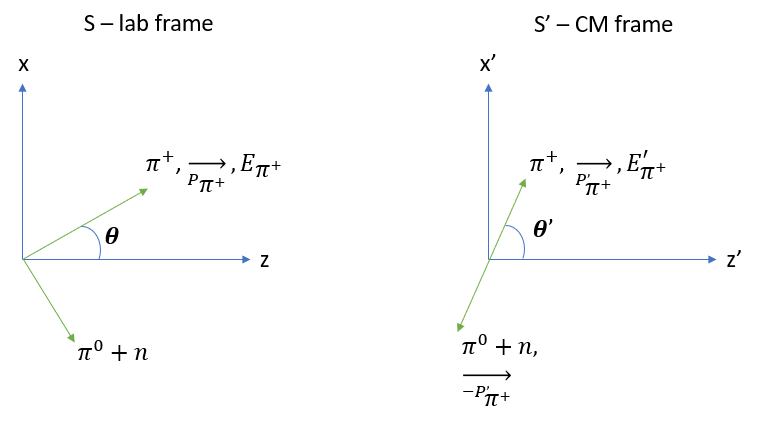
\includegraphics[scale=0.75]{Images/kinematic_calc/lab and CM ref frames for polar angle pion prod.png}
    \caption{Pion production at a non zero polar angle. The relative motion between the lab and CM mass frame is same as in the case where the pion production is along the +Z direction shown in equations \ref{equ:V_CM} and \ref{equ:V_lab}}
    \label{fig:pion production at a polar angle}
\end{figure}

The magnitude of $\vec{P}'_{\pi^+}$ is same as given by equation:\ref{equ:piplus_momentum_2pi}. What we want to find is the maximum possible magnitude of $\vec{P}_{\pi^+}$. 
%\For convenience let's define,
%\begin{equation}
%   |\vec{P}'_{\pi^+}| = p'_{\pi^+}
%\end{equation}
%and
%\begin{equation}
%   |\vec{P}_{\pi^+}| = p_{\pi^+}
%\end{equation}
In terms of the x,y,z components $|\vec{P}_{\pi^+}|$ can be expressed as,
\begin{equation}
    |\vec{P}_{\pi^+}| = \sqrt{p_{\pi^+,x}^2 + p_{\pi^+,y}^2 + p_{\pi^+,z}^2}
    \label{p magnitude}
\end{equation}
But since we can choose the scattering plane to be perpendicular to the y axis, we have $p_{\pi^+,y}=0$. The x component is straightforward and the z component can be obtained from the Lorentz transformations, respectively as,
\begin{equation}
    p_{\pi^+,x} = p'_{\pi^+,x} = |\vec{P}'_{\pi^+}|\sin{\theta'}
    \label{p_x}
\end{equation}
\begin{equation}
    p_{\pi^+,z} = \gamma(p'_z + vE'_{\pi^+}) = \gamma(|\vec{P}'_{\pi^+}|\cos{\theta'} + vE'_{\pi^+})
    \label{p_z}
\end{equation}
Where $v = |\vec{V}_{lab}| = |\vec{V}_{CM}|$ .
%and $E'_{\pi^+}=E'$ for convenience.
By substituting into the equation:\ref{p magnitude} and after a little bit of algebra we get,
\begin{equation}
    |\vec{P}_{\pi^+}| = \sqrt{(\gamma^2-1)|\vec{P}'_{\pi^+}|^2\cos^2{\theta'} + 2\gamma^2|\vec{P}'_{\pi^+}|vE'_{\pi^+}\cos{\theta'} + |\vec{P}'_{\pi^+}|^2 + \gamma^2v^2E'^{2}_{\pi^+}}
    \label{equ: pi+ momentum magnitude in lab frame for polar angle case}
\end{equation}
 But we still need to express $\theta'$ in terms of the quantities we already know. The angle $\theta$ counts as a quantity we know as we want to find the maximum possible $\pi^+$ momentum for a given scattering angle $\theta$. Therefore, we can write,
 \begin{equation}
     \tan{\theta} = \frac{p_{\pi^+,x}}{p_{\pi^+,z}} = \frac{|\vec{P}'_{\pi^+}|\sin{\theta'}}{\gamma(|\vec{P}'_{\pi^+}|\cos{\theta'} + vE'_{\pi^+})}
 \end{equation}
 From which we can obtain a quadratic equation of $\cos{\theta'}$,
 \begin{equation}
     [(\gamma^2\tan^2{\theta} + 1)|\vec{P}'_{\pi^+}|^2]\cos^2{\theta'} + [2vE'_{\pi^+}|\vec{P}'_{\pi^+}|\gamma^2\tan^2{\theta}]\cos{\theta'} + [\gamma^2\tan^2{\theta}v^2E'^{2}_{\pi^+}-|\vec{P}'_{\pi^+}|^2] = 0
 \end{equation}
 and solving for $\cos{\theta'}$ we get,
 % \begin{equation}
 %    \cos{\theta'} = \frac{-vE'_{\pi^+}|\vec{P}'_{\pi^+}|\gamma^2\tan^2{\theta} \pm \sqrt{\gamma^2\tan^2{\theta}(|\vec{P}'_{\pi^+}|^2-v^2E'^{2}_{\pi^+})+|\vec{P}'_{\pi^+}|^2}}{|\vec{P}'_{\pi^+}|(\gamma^2\tan^2{\theta} + 1)}
 % \end{equation} % This was the formula with an error -> extra |\vec{P}'_{\pi^+}| term in the left term of the numerator.

  \begin{equation}
    \cos{\theta'} = \frac{-vE'_{\pi^+}\gamma^2\tan^2{\theta} \pm \sqrt{\gamma^2\tan^2{\theta}(|\vec{P}'_{\pi^+}|^2-v^2E'^{2}_{\pi^+})+|\vec{P}'_{\pi^+}|^2}}{|\vec{P}'_{\pi^+}|(\gamma^2\tan^2{\theta} + 1)}
 \end{equation}

Substituting back into the equation:\ref{equ: pi+ momentum magnitude in lab frame for polar angle case}, we can find $|\vec{P}'_{\pi^+}|$. Since it is not obvious for what solution of $\cos{\theta'}$ we get the largest value for $|\vec{P}'_{\pi^+}|$, for each $\theta$ (kinematic setting) I had to evaluate both values and see. In all the cases, the positive solution gave the larger value.
% In all cases, I got a negative, smaller than -1 (so a -1.xxx number) for $\cos{\theta'}$ when I considered the negative solution which is invalid ($-1 \leq \cos{\theta} \leq +1$). Therefore, we will have to stick with the positive solution, which I checked to be always a valid value.


\subsection{Threshold Calculation Results}

The following figure:\ref{fig:table4 from GMn proposal} shows pion production thresholds for 3 different kinematic values which are shown in the very first G$_M^n$ proposal (Table:4 in page 30). All the values are explained in the text below the table itself. In table:\ref{Threshold calculation results table}, which resembles the table from the proposal, we present our calculation results. The first 6 columns of table:\ref{Threshold calculation results table} follows from the formalism we have explained in the earlier sections (above I have given formalism for max momenta but the conversion to energy is straight forward) and we will explain how the calculation of $E^{min}_\gamma$ was done in the section \ref{sec:E_gamma_min}.

\begin{figure}[h!]
    \centering
    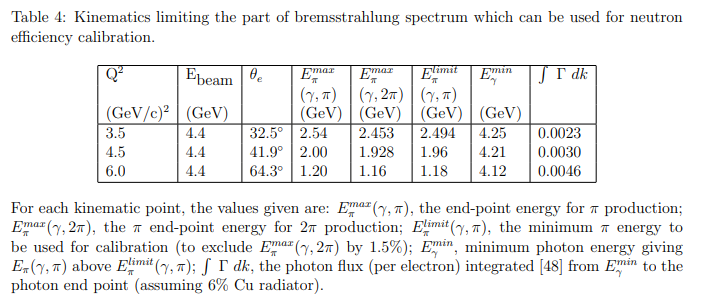
\includegraphics{Images/kinematic_calc/Table4-GMn original proposal.png}
    \caption{Pion production threshold calculations from the original $G_M^n$ proposal}
    \label{fig:table4 from GMn proposal}
\end{figure}


\begin{table}[h!]
    \centering
    \resizebox{1\textwidth}{!}{
    \begin{tabular}{|p{2cm}|p{2cm}|p{1cm}|p{2cm}|p{2cm}|p{2cm}|p{2cm}|}
    \hline
    %Q$^2$ (GeV/c)$^2$ & $E_{beam}$ (GeV) & $\theta_e$ & $E^{max}_{\pi} (\gamma,\pi)$ (GeV) & $E^{max}_{\pi}(\gamma,2\pi)$ (GeV) & $E^{limit}_{\pi}(\gamma,\pi)$ (GeV) & $E^{min}_\gamma$ (GeV) \\
    Q$^2$ \newline (GeV/c)$^2$ & $E_{beam}$ \newline (GeV) & $\theta_e$ & $E^{max}_{\pi}$ \newline $(\gamma,\pi)$ \newline (GeV) & $E^{max}_{\pi}$ \newline$(\gamma,2\pi)$ \newline(GeV) & $E^{limit}_{\pi}$ \newline$(\gamma,\pi)$ \newline(GeV) & $E^{min}_\gamma$ \newline(GeV) \\
    \hline
    3.5 & 4.4 & $32.5^o$ & 2.533 & 2.450 & 2.486 & 4.260 \\
    4.5 & 4.4 & $41.9^o$ & 1.997 & 1.931 & 1.960 & 4.224 \\
    6.0 & 4.4 & $64.3^o$ & 1.202 & 1.162 & 1.179 & 4.114 \\
    \hline    
    \end{tabular}
    }
    %\caption{Kinematics limiting the part of the bremsstrahlung spectrum which can be used for neutron efficiency calibration - Results I obtained}
    \caption{Results I obtained for the same input parameters as in the proposal}
    \label{Threshold calculation results table}
\end{table}

\subsection{Finding  $E^{min}_\gamma$}\label{sec:E_gamma_min}
 $E^{min}_\gamma$ is the minimum photon energy required to produce $\pi^+$ above $E^{limit}_{\pi}(\gamma,\pi)$. According to the description given in figure \ref{fig:table4 from GMn proposal},

 \begin{equation}
    E^{limit}_{\pi} = E^{max}_{\pi}(\gamma,2\pi).(1 + 1.5\%)
 \end{equation}

% and from that we can calculate the momentum limit $|\vec{P}^{limit}_{\pi}|$ as,
% \begin{equation}
%     |\vec{P}^{limit}_{\pi}| = \sqrt{ (E^{limit}_{\pi})^2 - m_{\pi^+}^2 }
% \end{equation}
% Lorentz transforming the energy back into the CM frame we get,
% \begin{equation}
%     (E^{limit}_{\pi^+})' = \gamma(E^{limit}_{\pi} - v\vec|{P}^{limit}_{\pi}|\cos{\theta})
% \end{equation}
% and 
% \begin{equation}
%     |(\vec{P}^{limit}_{\pi^+})'| = \sqrt{ ((E^{limit}_{\pi^+})')^2  - m_{\pi^+}^2 }
% \end{equation}

% Now from equation \ref{equ: Mandelstam s in lab fram} and \ref{equ: Mandelstam s in CM frame}, we can solve for $E_\gamma$, since we know $|(\vec{P}^{limit}_{\pi})'|$.
% \begin{equation}
%   E^{min}_\gamma  = \frac{ \left(\sqrt{m_n^2 + |(\vec{P}^{limit}_{\pi^+})'|^2} + \sqrt{m^2_{\pi^+} + |(\vec{P}^{limit}_{\pi^+})'|^2})\right)^2 - m_p^2}{2m_p}
% \end{equation}

Once you know the $\pi^+$ momentum in the lab frame, you can calculate the photon energy of the reaction $p(\gamma,\pi^+)n$, using the first principles. Using the conservation of four-momentum, we can write:

\begin{equation}
    p_\gamma^\mu + p_p^\mu = p_{\pi^+}^\mu + p_n^\mu
\end{equation}

By solving for $p_n^\mu$ and taking the invariant dot product of both sides we get:
\begin{equation}
    m_p^2 + 2E_{\gamma}m_p + m_{\pi^+}^2 -2[E_{\gamma}E_{\pi^+} - E_{\gamma}p_{\pi^+}\cos{\theta} + E_{\pi^+}m_p] = m_n^2 
\end{equation}
Then we can simply solve for the photon energy:
\begin{equation}\label{equ:  photonE_formula}
    E_{\gamma} = \frac{ 2m_pE_{\pi^+} + m_n^2 - m_{\pi^+}^2 - m_p^2 }{ 2( m_p + p_{\pi^+}\cos{\theta} - E_{\pi^+} ) }
\end{equation}

Thus, when we know the $\pi^+$ track momentum from BigBite, we can find the photon energy for the reaction $p(\gamma,\pi^+)n$. This can be used to find $E^{min}_\gamma$.


\subsection{Threshold calculations for all the actual $G_M^n$ kinematic points we took data}

Now we can extend the above calculations to the actual $G_M^n$ experiment's kinematic points. In addition to the above parameters, I am including the HCal angle and the expected $\pi^+$ polar angle for the reaction $\gamma(p,\pi^+)n$. When calculating the $\pi^+$ polar angle, I am assuming the photon energy to be equal to the beam energy. It can be seen that the kinematics of the $\gamma(p,\pi^+)n$ reaction follows very closely with the elastic scattering kinematics. See table:\ref{Table: Threshold calculation results for the actual GMn kinematics}.

\begin{table}[h!]
    \centering
    \resizebox{1\textwidth}{!}{
    \begin{tabular}{|p{1.5cm}|p{2cm}|p{2cm}|p{1cm}|p{1cm}|p{1.5cm}|p{2cm}|p{2cm}|p{2cm}|p{2cm}|}
    \hline
    Kin num & Q$^2$ \newline (GeV/c)$^2$ & $E_{beam}$ \newline (GeV) & $\theta_e$ (deg) & HCal \newline angle \newline (deg) & neutron angle \newline $p(\gamma,\pi^+)n$ \newline (deg) & $E^{max}_{\pi}$ \newline $(\gamma,\pi)$ \newline (GeV) & $E^{max}_{\pi}$ \newline$(\gamma,2\pi)$ \newline(GeV) & $E^{limit}_{\pi}$ \newline$(\gamma,\pi)$ \newline(GeV) & $E^{min}_\gamma$ \newline(GeV) \\
    \hline
    SBS 4 & 3.0 & 3.7393 & 36.0 & 31.9 & 31.5 & 2.120 & 2.037 & 2.068 & 3.581 \\
    SBS 8 & 4.5 & 5.9826 & 26.5 & 29.4 & 30.1 & 3.579 & 3.492 & 3.544 & 5.887 \\
    \rowcolor{blue!20} SBS 9 & 4.5 & 4.0268 & 49.0 & 22.0 & 22.6 & 1.623 & 1.564 & 1.588 & 3.816 \\
    SBS 14 & 7.5 & 5.9828 & 46.5 & 17.0 & 17.7 & 1.999 & 1.950 & 1.979 & 5.812 \\
    SBS 7 & 10 & 7.9308 & 40.0 & 16.1 & 16.5 & 2.659 & 2.610 & 2.649 & 7.846 \\
    SBS 11 & 13.6 & 9.889 & 42 & 13.3 & 12.8 & 2.662 & 2.623 & 2.662 & 9.891 \\
    \rowcolor{red!20} SBS 12 & 4.5 & 4.3 & 42.5 & 25.9 & 25.6 & 1.947 & 1.881 & 1.910 & 4.120 \\  
    \hline
    \end{tabular}
    }
    \caption{Threshold calculations for the actual $G_M^n$ experiment's kinematic points}
    \label{Table: Threshold calculation results for the actual GMn kinematics}
\end{table}

The SBS 9 kinematic point is highlighted in light-blue, which we are currently analyzing and we think that has highest prospects in succeeding this analysis, due to the lowest $\pi^+$ momentum. The GEn-RP kinematic point (SBS 12), is highlighted in light-red. Discussions are ongoing to utilize this GEn-RP kinematic point to collect some dedicated data for neutron detection efficiency calibrations with the following conditions:
\begin{itemize}
    \item Use LH2 target
    \item Use a copper radiator
    \item BigBite magnet run in reverse (positive) polarity so that the $\pi^+$ will be bent in the upward direction
    \item Remove steel analyzer from the GEn-RP inline stack
    \item Any other requirements?
\end{itemize}


